% !TEX encoding = UTF-8 Unicode
%!TEX root = thesis.tex
% !TEX spellcheck = en-US
%%=========================================
\section{Experiment 1}
In this experiment, the aim is to find a good combination of crossover rate and mutation rate.

\subsection{Configuration}
\begin{minipage}{\linewidth}
\centering
\captionof{table}{Table Title TODO} \label{tab:title} 
\begin{tabular}{ C{3.5in} C{1.6in} }\toprule[1.5pt]
\bf Parameter & \bf Value \\
\midrule
  Number of generations & 20 \\
\midrule
  Fitness function & Local similarity \\
\midrule
  Target sound & Drum loop \\
\midrule
  Input sound & White noise \\
\midrule
  Effect & Distortion and resonant low-pass filter \\
\midrule
  Audio features & mfcc\_0, mfcc\_0\_\_derivative, mfcc\_1 \\
\midrule
  Number of runs & 250 per configuration \\
\bottomrule[1.25pt]
\end {tabular}\par
\bigskip
Should be a caption TODO
\end{minipage}

\subsection{Fitness function}
The local similarity fitness function is based on the average euclidean distance between the feature vector of the target sound and the output sound in the k frames of the two sounds.

\begin{verbatim}
Function LOCAL_SIMILARITY(target, individual):
    total_euclidean_distance = 0
    for each k in range(num_frames):
        A = target.get_feature_vector(k)
        C = individual.get_feature_vector(k)
        total_euclidean_distance += EUCLIDEAN_DISTANCE(A, C)
    avg_euclidean_distance = total_euclidean_distance / num_frames
    return 1 / (1 + avg_euclidean distance)
\end{verbatim}

where \texttt{EUCLIDEAN\_DISTANCE} is $d(p,q)=\sqrt{(q_1-p_1)^2+(q_2-p_2)+...+(q_n-p_n)^2}$

\subsection{Evaluation of configurations}
Figure 4.1 TODO shows that ...

\begin{figure}[h]
    \centering
    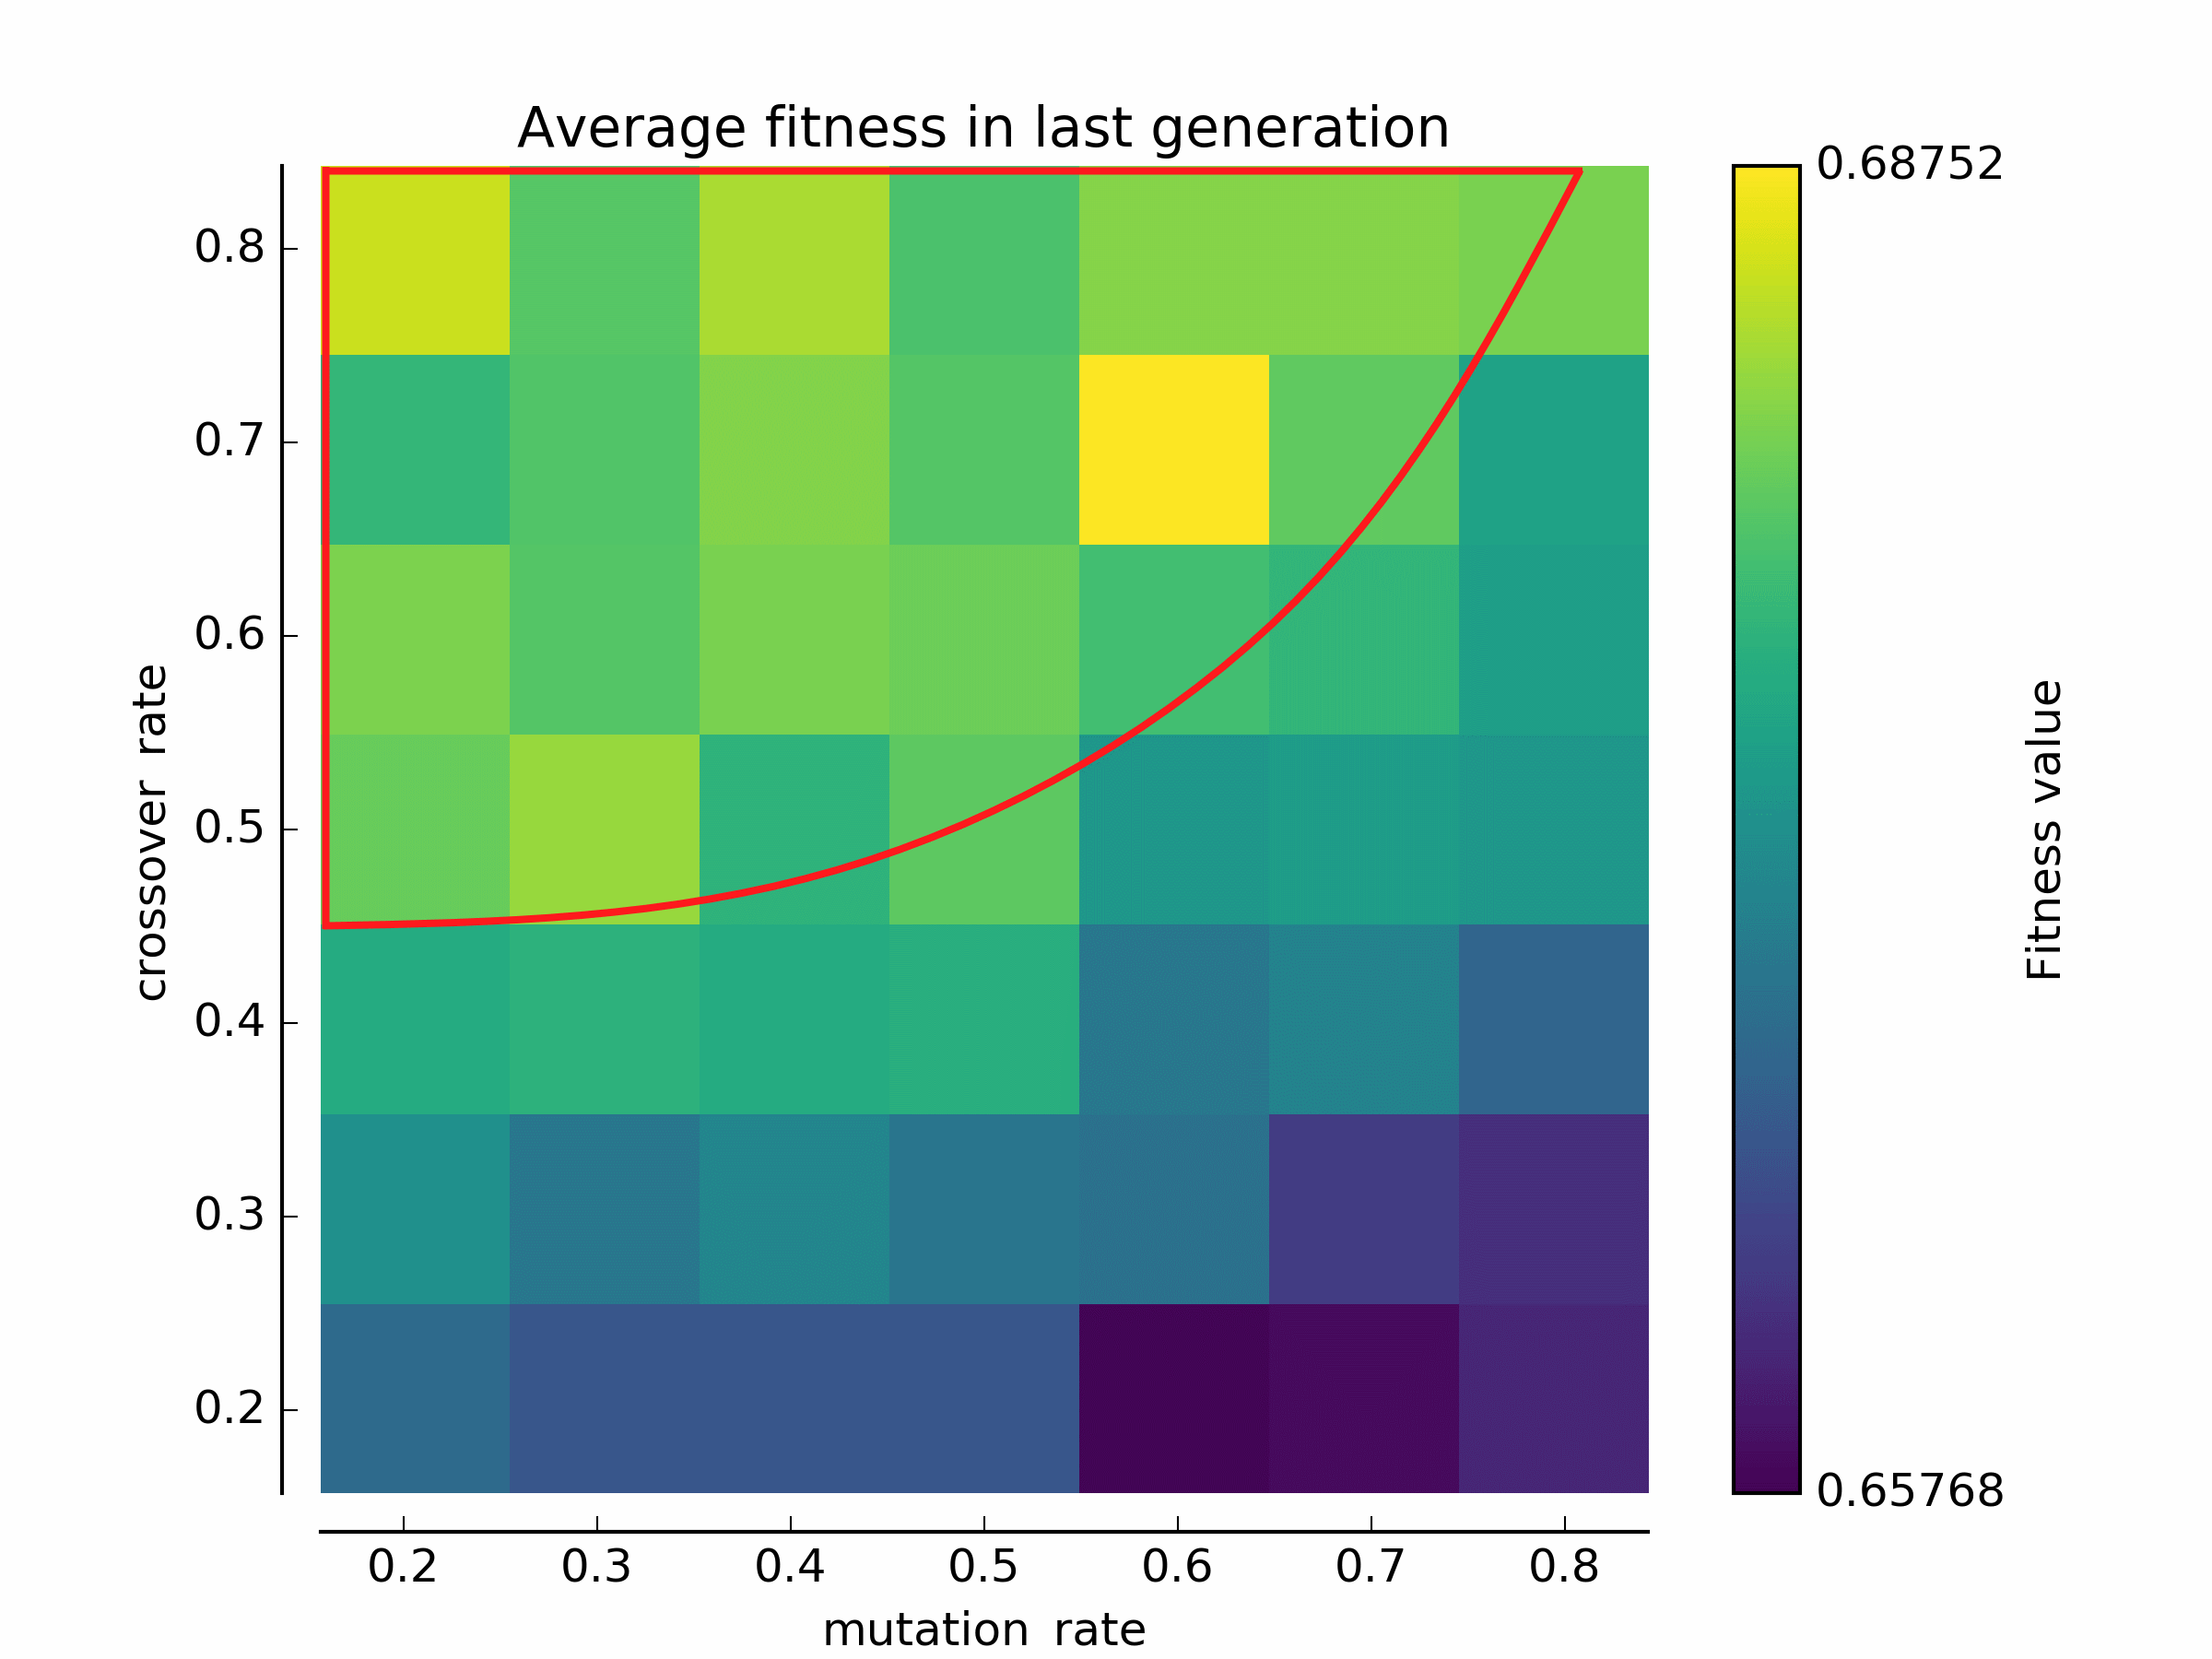
\includegraphics[width=0.99\textwidth]{grid_search_crossover_mutation_avg}
    \caption{TODO caption}
    \label{fig:grid_search_crossover_mutation_avg}
\end{figure}
